\subsection{Basics}
\label{subsec:basics-passive}

Let's dive into the fundamental components that make up the backbone of any electronic circuit. These components are like the essential workers of the electronics world—often overlooked but absolutely essential. We'll start with resistors, capacitors, inductors, and switches, and then move on to some battery chemistry basics. By the end of this section, you'll have a solid understanding of how these components work and why they're so important.



\begin{figure}[h!]
    \centering
    \footnotesize
    \begin{tabular}{ccccc}
        % Row 1 - Resistive and Protection Components
        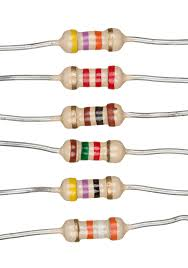
\includegraphics[width=0.11\textwidth]{images/resistor} &
        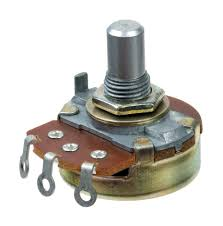
\includegraphics[width=0.11\textwidth]{images/potentiometer} &
        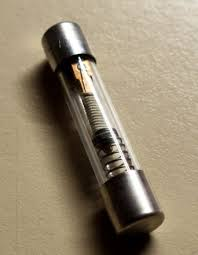
\includegraphics[width=0.11\textwidth]{images/fuse} &
        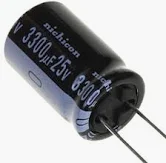
\includegraphics[width=0.11\textwidth]{images/capacitor} &
        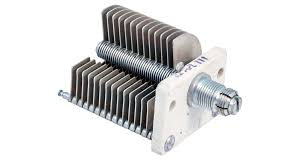
\includegraphics[width=0.11\textwidth]{images/variable-capacitor} \\
        Through-hole Resistor & Potentiometer & Glass Fuse & Ceramic Capacitor & Variable Capacitor \\[2em]
        % Row 2 - Inductors and Switches
        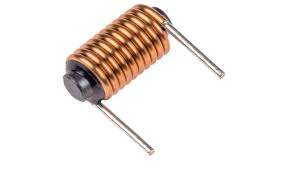
\includegraphics[width=0.11\textwidth]{images/inductor} &
        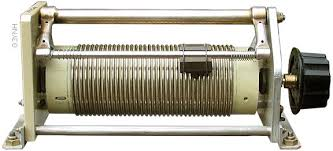
\includegraphics[width=0.11\textwidth]{images/variable-inductor} &
        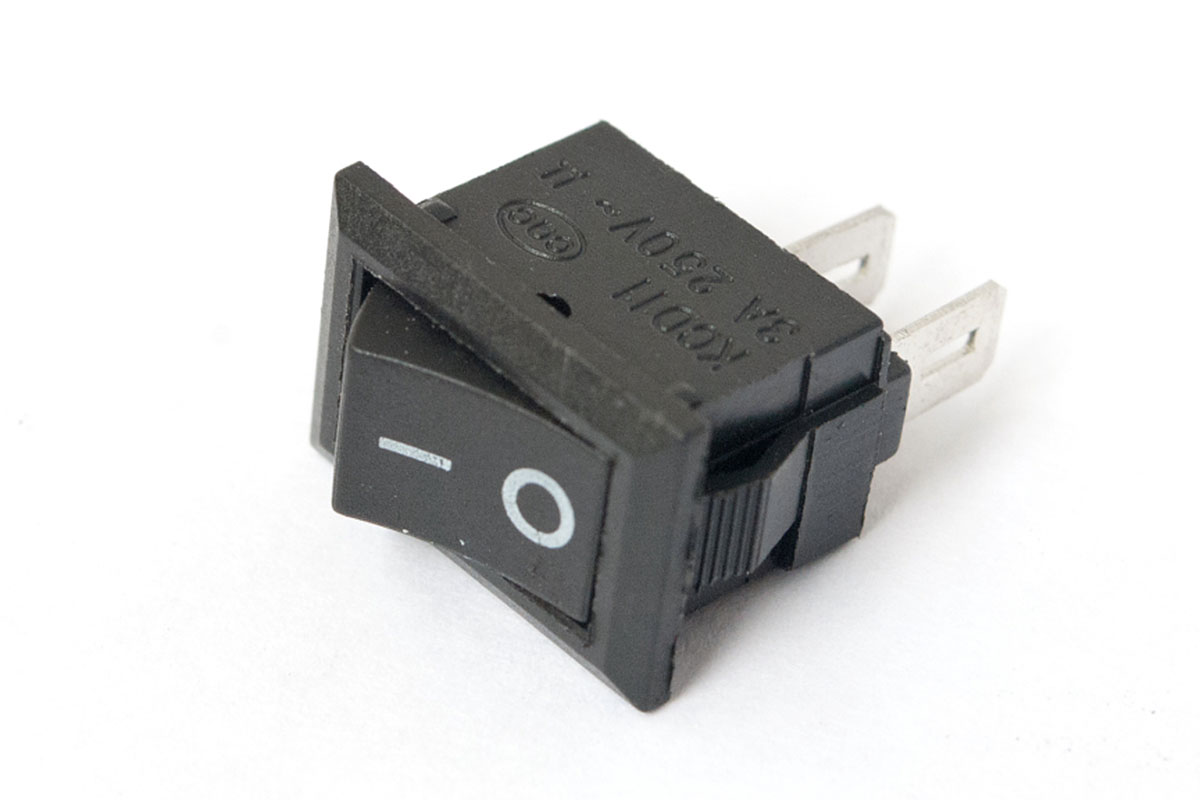
\includegraphics[width=0.11\textwidth]{images/spst} &
        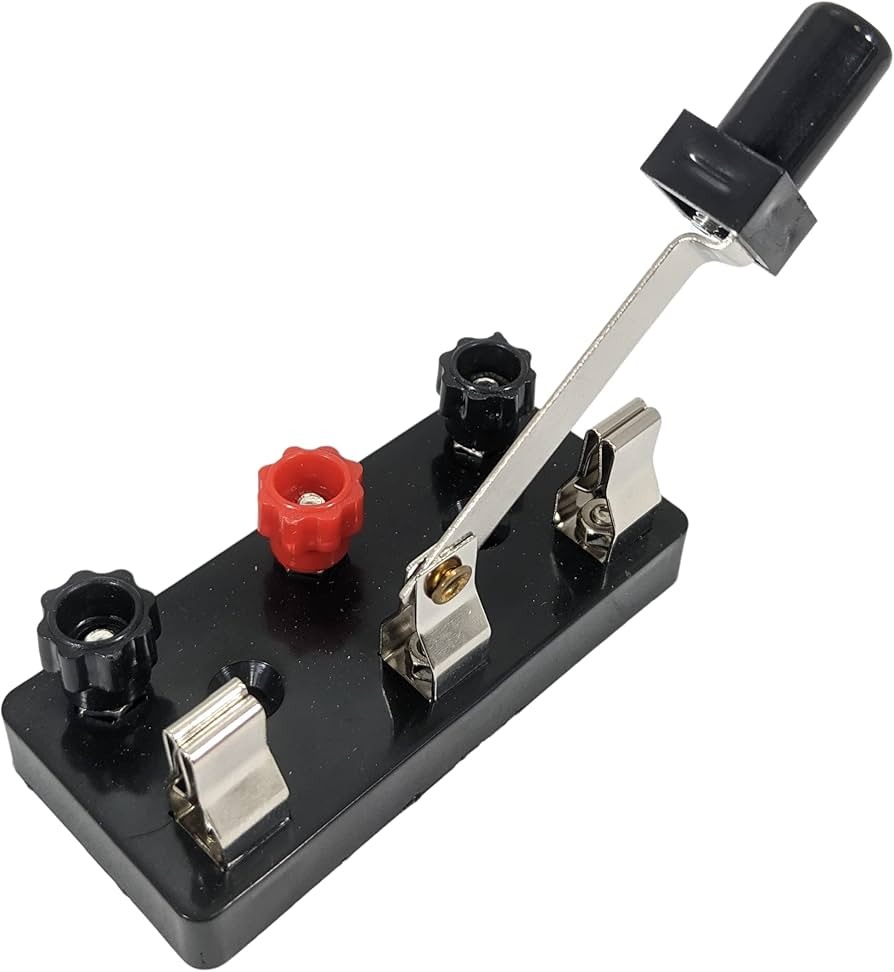
\includegraphics[width=0.11\textwidth]{images/spdt} & \\
        Toroid Inductor & Variable Inductor & SPST Switch & SPDT Switch & \\
    \end{tabular}
    \caption{Common electronic components used in radio circuits. Top row: fixed resistor with color-coded bands, potentiometer for variable resistance, glass fuse for circuit protection, fixed ceramic capacitor, and variable capacitor for tuning. Bottom row: toroidal inductor, variable inductor for RF adjustments, SPST switch for on/off control, and SPDT switch for selecting between two circuits.}
    \label{fig:component-photos}
\end{figure}


\subsubsection*{Resistors: The Traffic Cops of Current}
A resistor is like the traffic cop of a DC circuit—it controls the flow of current. When current tries to flow through a resistor, it faces opposition, which we call resistance. This opposition is measured in ohms ($\Omega$). The higher the resistance, the harder it is for current to flow. This relationship is described by Ohm's Law (Equation~\ref{eq:ohms-law}).

\subsubsection*{Potentiometers: The Volume Knob}
Ever wondered how the volume knob on your stereo works? That's a potentiometer in action! A potentiometer is essentially a variable resistor. It has three terminals: two fixed ends and a movable wiper. By adjusting the wiper, you can change the resistance between the wiper and one of the fixed ends. This is how you control the volume—by adjusting the resistance, you control the amount of current flowing through the circuit, which in turn controls the volume.

\subsubsection*{Capacitors: The Energy Storage Tanks}
Capacitors are like tiny energy storage tanks. They store energy in an electric field between two conductive plates separated by an insulator (called a dielectric). The amount of energy a capacitor can store is determined by its capacitance, measured in farads (F). The basic formula for capacitance is:
\begin{equation}
    C = \frac{Q}{V}
\end{equation}
where $C$ is capacitance, $Q$ is charge, and $V$ is voltage. Capacitors are used in a variety of applications, from filtering out noise in power supplies to timing circuits.

\subsubsection*{Inductors: The Magnetic Field Generators}
Inductors are the magnetic counterparts to capacitors. Instead of storing energy in an electric field, they store it in a magnetic field. An inductor is typically constructed as a coil of wire, and when current flows through it, a magnetic field is generated. The strength of this magnetic field depends on the inductance, measured in henries (H). Inductors are often used in filters and oscillators, where they help to smooth out current or generate specific frequencies.

\subsubsection*{SPDT Switches: The Circuit Directors}
An SPDT (Single-Pole Double-Throw) switch is like a railroad switch for circuits. It allows you to direct the flow of current between two different paths. Unlike a simple on/off switch, an SPDT switch can switch a single circuit between one of two other circuits. This makes it incredibly versatile for controlling complex circuits.

\subsubsection*{Fuses: The Circuit Protectors}
Fuses are critical safety components in electronic circuits. They are designed to break the circuit if the current exceeds a certain level, thereby protecting other components from damage. Think of them as the circuit's emergency brake. When too much current flows through a fuse, the wire inside it melts, breaking the circuit and stopping the flow of current.

\subsubsection*{Battery Chemistries: The Power Source}
Batteries come in all shapes and sizes, but they can be broadly categorized into rechargeable and non-rechargeable types. Rechargeable batteries, like Nickel-Metal Hydride (NiMH), Lithium-Ion (Li-ion), and Lead-Acid, can be recharged multiple times, making them more cost-effective and environmentally friendly in the long run. Non-rechargeable batteries, like Carbon-Zinc, are typically used in low-drain devices and are disposed of after use.

\subsubsection*{Single-Pole Single-Throw Switches: The Simplest Switch}
A Single-Pole Single-Throw (SPST) switch is the simplest type of switch. It has two terminals and can either open or close a single circuit. When the switch is closed, current flows; when it's open, the circuit is broken. It's the most basic form of switch and is used in a wide variety of applications.

\begin{table}[h!]
    \centering
    \caption{Comparison of Resistors, Capacitors, and Inductors}
    \label{tab:resistor-capacitor-inductor-comparison}
    \begin{tabular}{|l|l|l|l|}
        \hline
        \textbf{Component} & \textbf{Function} & \textbf{Energy Storage} & \textbf{Unit} \\
        \hline
        Resistor & Opposes current flow & None & Ohms ($\Omega$) \\
        Capacitor & Stores energy in electric field & Electric field & Farads (F) \\
        Inductor & Stores energy in magnetic field & Magnetic field & Henries (H) \\
        \hline
    \end{tabular}
\end{table}

\begin{table}[h!]
    \centering
    \caption{Common Battery Chemistries}
    \label{tab:battery-chemistries}
    \begin{tabular}{|l|l|l|}
        \hline
        \textbf{Chemistry} & \textbf{Rechargeable} & \textbf{Common Uses} \\
        \hline
        Nickel-Metal Hydride (NiMH) & Yes & Rechargeable batteries \\
        Lithium-Ion (Li-ion) & Yes & Smartphones, laptops \\
        Lead-Acid & Yes & Car batteries \\
        Carbon-Zinc & No & Low-drain devices \\
        \hline
    \end{tabular}
\end{table}


\subsubsection{Questions}

\begin{tcolorbox}[colback=gray!10!white,colframe=black!75!black,title={T6A01}]
    What electrical component opposes the flow of current in a DC circuit?
    \begin{enumerate}[label=\Alph*),noitemsep]
        \item Inductor
        \item \textbf{Resistor}
        \item Inverter
        \item Transformer
    \end{enumerate}
\end{tcolorbox}
A resistor opposes the flow of current in a DC circuit. Inductors and capacitors also affect current flow, but in different ways—inductors oppose changes in current, while capacitors store energy in an electric field.

\begin{tcolorbox}[colback=gray!10!white,colframe=black!75!black,title={T6A02}]
    What type of component is often used as an adjustable volume control?
    \begin{enumerate}[label=\Alph*),noitemsep]
        \item Fixed resistor
        \item Power resistor
        \item \textbf{Potentiometer}
        \item Transformer
    \end{enumerate}
\end{tcolorbox}
A potentiometer is often used as an adjustable volume control. It allows you to vary the resistance, which in turn adjusts the volume.

\begin{tcolorbox}[colback=gray!10!white,colframe=black!75!black,title={T6A03}]
    What electrical parameter is controlled by a potentiometer?
    \begin{enumerate}[label=\Alph*),noitemsep]
        \item Inductance
        \item \textbf{Resistance}
        \item Capacitance
        \item Field strength
    \end{enumerate}
\end{tcolorbox}
A potentiometer controls resistance. By adjusting the wiper, you can change the resistance between the wiper and one of the fixed ends.

\begin{tcolorbox}[colback=gray!10!white,colframe=black!75!black,title={T6A04}]
    What electrical component stores energy in an electric field?
    \begin{enumerate}[label=\Alph*),noitemsep]
        \item Varistor
        \item \textbf{Capacitor}
        \item Inductor
        \item Diode
    \end{enumerate}
\end{tcolorbox}
A capacitor stores energy in an electric field. Inductors store energy in a magnetic field, while varistors and diodes have different functions altogether.

\begin{tcolorbox}[colback=gray!10!white,colframe=black!75!black,title={T6A05}]
    What type of electrical component consists of conductive surfaces separated by an insulator?
    \begin{enumerate}[label=\Alph*),noitemsep]
        \item Resistor
        \item Potentiometer
        \item Oscillator
        \item \textbf{Capacitor}
    \end{enumerate}
\end{tcolorbox}
A capacitor consists of conductive surfaces separated by an insulator. This structure allows it to store energy in an electric field.

\begin{tcolorbox}[colback=gray!10!white,colframe=black!75!black,title={T6A06}]
    What type of electrical component stores energy in a magnetic field?
    \begin{enumerate}[label=\Alph*),noitemsep]
        \item Varistor
        \item Capacitor
        \item \textbf{Inductor}
        \item Diode
    \end{enumerate}
\end{tcolorbox}
An inductor stores energy in a magnetic field. Capacitors store energy in an electric field, while varistors and diodes have different functions.

\begin{tcolorbox}[colback=gray!10!white,colframe=black!75!black,title={T6A07}]
    What electrical component is typically constructed as a coil of wire?
    \begin{enumerate}[label=\Alph*),noitemsep]
        \item Switch
        \item Capacitor
        \item Diode
        \item \textbf{Inductor}
    \end{enumerate}
\end{tcolorbox}
An inductor is typically constructed as a coil of wire. This coil generates a magnetic field when current flows through it.

\begin{tcolorbox}[colback=gray!10!white,colframe=black!75!black,title={T6A08}]
    What is the function of an SPDT switch?
    \begin{enumerate}[label=\Alph*),noitemsep]
        \item A single circuit is opened or closed
        \item Two circuits are opened or closed
        \item \textbf{A single circuit is switched between one of two other circuits}
        \item Two circuits are each switched between one of two other circuits
    \end{enumerate}
\end{tcolorbox}
An SPDT switch allows a single circuit to be switched between one of two other circuits. This makes it useful for directing current flow in complex circuits.

\begin{tcolorbox}[colback=gray!10!white,colframe=black!75!black,title={T6A09}]
    What electrical component is used to protect other circuit components from current overloads?
    \begin{enumerate}[label=\Alph*),noitemsep]
        \item \textbf{Fuse}
        \item Thyratron
        \item Varactor
        \item All these choices are correct
    \end{enumerate}
\end{tcolorbox}
A fuse is used to protect other circuit components from current overloads. When the current exceeds a certain level, the fuse breaks the circuit, preventing damage.

\begin{tcolorbox}[colback=gray!10!white,colframe=black!75!black,title={T6A10}]
    Which of the following battery chemistries is rechargeable?
    \begin{enumerate}[label=\Alph*),noitemsep]
        \item Nickel-metal hydride
        \item Lithium-ion
        \item Lead-acid
        \item \textbf{All these choices are correct}
    \end{enumerate}
\end{tcolorbox}
All the listed battery chemistries—Nickel-Metal Hydride, Lithium-Ion, and Lead-Acid—are rechargeable. They can be recharged multiple times, making them more cost-effective and environmentally friendly.

\begin{tcolorbox}[colback=gray!10!white,colframe=black!75!black,title={T6A11}]
    Which of the following battery chemistries is not rechargeable?
    \begin{enumerate}[label=\Alph*),noitemsep]
        \item Nickel-cadmium
        \item \textbf{Carbon-zinc}
        \item Lead-acid
        \item Lithium-ion
    \end{enumerate}
\end{tcolorbox}
Carbon-Zinc batteries are not rechargeable. They are typically used in low-drain devices and are disposed of after use.

\begin{tcolorbox}[colback=gray!10!white,colframe=black!75!black,title={T6A12}]
    What type of switch is represented by component 3 in figure T-2?
    \begin{enumerate}[label=\Alph*),noitemsep]
        \item \textbf{Single-pole single-throw}
        \item Single-pole double-throw
        \item Double-pole single-throw
        \item Double-pole double-throw
    \end{enumerate}
\end{tcolorbox}
Component 3 in figure T-2 represents a Single-Pole Single-Throw (SPST) switch. This type of switch is the simplest, allowing a single circuit to be opened or closed.
